%%
%% Beginning of file 'sample62.tex'
%%
%% Modified 2018 January
%%
%% This is a sample manuscript marked up using the
%% AASTeX v6.2 LaTeX 2e macros.
%%
%% AASTeX is now based on Alexey Vikhlinin's emulateapj.cls 
%% (Copyright 2000-2015).  See the classfile for details.

%% AASTeX requires revtex4-1.cls (http://publish.aps.org/revtex4/) and
%% other external packages (latexsym, graphicx, amssymb, longtable, and epsf).
%% All of these external packages should already be present in the modern TeX 
%% distributions.  If not they can also be obtained at www.ctan.org.

%% The first piece of markup in an AASTeX v6.x document is the \documentclass
%% command. LaTeX will ignore any data that comes before this command. The 
%% documentclass can take an optional argument to modify the output style.
%% The command below calls the preprint style  which will produce a tightly 
%% typeset, one-column, single-spaced document.  It is the default and thus
%% does not need to be explicitly stated.
%%
%%
%% using aastex version 6.2
\documentclass[trackchanges, floatfix, twocolumn, tighten]{aastex62}

%% The default is a single spaced, 10 point font, single spaced article.
%% There are 5 other style options available via an optional argument. They
%% can be envoked like this:
%%
%% \documentclass[argument]{aastex62}
%% 
%% where the layout options are:
%%
%%  twocolumn   : two text columns, 10 point font, single spaced article.
%%                This is the most compact and represent the final published
%%                derived PDF copy of the accepted manuscript from the publisher
%%  manuscript  : one text column, 12 point font, double spaced article.
%%  preprint    : one text column, 12 point font, single spaced article.  
%%  preprint2   : two text columns, 12 point font, single spaced article.
%%  modern      : a stylish, single text column, 12 point font, article with
%% 		  wider left and right margins. This uses the Daniel
%% 		  Foreman-Mackey and David Hogg design.
%%  RNAAS       : Preferred style for Research Notes which are by design 
%%                lacking an abstract and brief. DO NOT use \begin{abstract}
%%                and \end{abstract} with this style.
%%
%% Note that you can submit to the AAS Journals in any of these 6 styles.
%%
%% There are other optional arguments one can envoke to allow other stylistic
%% actions. The available options are:
%%
%%  astrosymb    : Loads Astrosymb font and define \astrocommands. 
%%  tighten      : Makes baselineskip slightly smaller, only works with 
%%                 the twocolumn substyle.
%%  times        : uses times font instead of the default
%%  linenumbers  : turn on lineno package.
%%  trackchanges : required to see the revision mark up and print its output
%%  longauthor   : Do not use the more compressed footnote style (default) for 
%%                 the author/collaboration/affiliations. Instead print all
%%                 affiliation information after each name. Creates a much
%%                 long author list but may be desirable for short author papers
%%
%% these can be used in any combination, e.g.
%%
%% \documentclass[twocolumn,linenumbers,trackchanges]{aastex62}
%%
%% AASTeX v6.* now includes \hyperref support. While we have built in specific
%% defaults into the classfile you can manually override them with the
%% \hypersetup command. For example,
%%
%%\hypersetup{linkcolor=red,citecolor=green,filecolor=cyan,urlcolor=magenta}
%%
%% will change the color of the internal links to red, the links to the
%% bibliography to green, the file links to cyan, and the external links to
%% magenta. Additional information on \hyperref options can be found here:
%% https://www.tug.org/applications/hyperref/manual.html#x1-40003
%%
%% If you want to create your own macros, you can do so
%% using \newcommand. Your macros should appear before
%% the \begin{document} command.
%%
\newcommand{\vdag}{(v)^\dagger}
\newcommand\aastex{AAS\TeX}
\newcommand\latex{La\TeX}

%% Reintroduced the \received and \accepted commands from AASTeX v5.2
\received{June 22, 2019}
\revised{August 18, 2019}
\accepted{August 30, 2019}
%% Command to document which AAS Journal the manuscript was submitted to.
%% Adds "Submitted to " the arguement.
\submitjournal{AJ}

%% Mark up commands to limit the number of authors on the front page.
%% Note that in AASTeX v6.2 a \collaboration call (see below) counts as
%% an author in this case.
%
%\AuthorCollaborationLimit=3
%
%% Will only show Schwarz, Muench and "the AAS Journals Data Scientist 
%% collaboration" on the front page of this example manuscript.
%%
%% Note that all of the author will be shown in the published article.
%% This feature is meant to be used prior to acceptance to make the
%% front end of a long author article more manageable. Please do not use
%% this functionality for manuscripts with less than 20 authors. Conversely,
%% please do use this when the number of authors exceeds 40.
%%
%% Use \allauthors at the manuscript end to show the full author list.
%% This command should only be used with \AuthorCollaborationLimit is used.

%% The following command can be used to set the latex table counters.  It
%% is needed in this document because it uses a mix of latex tabular and
%% AASTeX deluxetables.  In general it should not be needed.
%\setcounter{table}{1}

%%%%%%%%%%%%%%%%%%%%%%%%%%%%%%%%%%%%%%%%%%%%%%%%%%%%%%%%%%%%%%%%%%%%%%%%%%%%%%%%
%%
%% The following section outlines numerous optional output that
%% can be displayed in the front matter or as running meta-data.
%%
%% If you wish, you may supply running head information, although
%% this information may be modified by the editorial offices.
\shorttitle{Automated MK Classification}
\shortauthors{Brice and Andonie}
%%
%% You can add a light gray and diagonal water-mark to the first page 
%% with this command:
% \watermark{text}
%% where "text", e.g. DRAFT, is the text to appear.  If the text is 
%% long you can control the water-mark size with:
%  \setwatermarkfontsize{dimension}
%% where dimension is any recognized LaTeX dimension, e.g. pt, in, etc.
%%
%%%%%%%%%%%%%%%%%%%%%%%%%%%%%%%%%%%%%%%%%%%%%%%%%%%%%%%%%%%%%%%%%%%%%%%%%%%%%%%%

%% This is the end of the preamble.  Indicate the beginning of the
%% manuscript itself with \begin{document}.

\usepackage{url}
\usepackage{verbatim}
\usepackage{multirow}
\usepackage{float}

%\usepackage{caption}

\usepackage{algorithm}
\usepackage{todonotes}
\usepackage{varwidth}% http://ctan.org/pkg/varwidth

\usepackage{algpseudocode}% http://ctan.org/pkg/algorithmicx
\newcommand{\vars}{\texttt}
\let\oldReturn\Return
\renewcommand{\Return}{\State\oldReturn}
\newcommand{\func}{\textrm}


\usepackage{hyperref}
% This sets up the hyperlink's colors
\hypersetup{linktocpage, 
    colorlinks,
    citecolor=blue,
    filecolor=blue,
    linkcolor=blue,
    urlcolor=blue}

\usepackage{savesym}
\savesymbol{tablenum}
\usepackage{siunitx}
\restoresymbol{SIX}{tablenum}


\pdfoutput=1 %for arXiv submission
\usepackage[T1]{fontenc}
%\usepackage{apjfonts} 
%\usepackage[figure,figure*]{hypcap}
\usepackage{url}
\usepackage[caption=false]{subfig}

\usepackage{lipsum} % just for the example

\usepackage{ifpdf}
\ifpdf
\usepackage{epstopdf}
\fi

\usepackage{multirow}
\usepackage{siunitx}
\usepackage{array,tikz}
\usepackage{soul}

\usetikzlibrary{tikzmark,arrows.meta}
% Spectra template example
\newcolumntype{M}{>{\centering\mbox{}\vfill\arraybackslash}m{50pt}<{\vfill}}

\newcommand{\RomanNumeralCaps}[1] {\MakeUppercase{\romannumeral #1}}

\newcommand{\specialcell}[2][l]{%
  \begin{tabular}[#1]{@{}l@{}}#2\end{tabular}}

\usepackage{array}% http://ctan.org/pkg/array

\usepackage{amsmath}
\newcommand\norm[1]{\left\lVert#1\right\rVert}
%\usepackage{cleveref}

% correct bad hyphenation here
\hyphenation{op-tical net-works semi-conduc-tor}
 
% Equation Numbers
%\renewcommand{\theequation}{\arabic{section}.\arabic{equation}}
\usepackage{chngcntr}

\usepackage{color}
%\DeclareRobustCommand{\hlcyan}[1]{{\sethlcolor{cyan}\hl{#1}}}
%\DeclareRobustCommand{\hlorange}[1]{{\sethlcolor{orange}\hl{#1}}}
%\counterwithin*{equation}{section}

\newcommand{\NA}{---}

\usepackage{subfiles}
\usepackage{rotating}
\usepackage{enumerate}

\usepackage{algorithm}% http://ctan.org/pkg/algorithms
\usepackage{algpseudocode}% http://ctan.org/pkg/algorithmicx


\begin{document}

\title{Automated MK Classification of Observed Stellar Spectra collected by the Sloan Digital Sky Survey using a Single Classifier\footnote{Released on TBD}}

%% LaTeX will automatically break titles if they run longer than
%% one line. However, you may use \\ to force a line break if
%% you desire. In v6.2 you can include a footnote in the title.

%% A significant change from earlier AASTEX versions is in the structure for 
%% calling author and affilations. The change was necessary to implement 
%% autoindexing of affilations which prior was a manual process that could 
%% easily be tedious in large author manuscripts.
%%
%% The \author command is the same as before except it now takes an optional
%% arguement which is the 16 digit ORCID. The syntax is:
%% \author[xxxx-xxxx-xxxx-xxxx]{Author Name}
%%
%% This will hyperlink the author name to the author's ORCID page. Note that
%% during compilation, LaTeX will do some limited checking of the format of
%% the ID to make sure it is valid.
%%
%% Use \affiliation for affiliation information. The old \affil is now aliased
%% to \affiliation. AASTeX v6.2 will automatically index these in the header.
%% When a duplicate is found its index will be the same as its previous entry.
%%
%% Note that \altaffilmark and \altaffiltext have been removed and thus 
%% can not be used to document secondary affiliations. If they are used latex
%% will issue a specific error message and quit. Please use multiple 
%% \affiliation calls for to document more than one affiliation.
%%
%% The new \altaffiliation can be used to indicate some secondary information
%% such as fellowships. This command produces a non-numeric footnote that is
%% set away from the numeric \affiliation footnotes.  NOTE that if an
%% \altaffiliation command is used it must come BEFORE the \affiliation call,
%% right after the \author command, in order to place the footnotes in
%% the proper location.
%%
%% Use \email to set provide email addresses. Each \email will appear on its
%% own line so you can put multiple email address in one \email call. A new
%% \correspondingauthor command is available in V6.2 to identify the
%% corresponding author of the manuscript. It is the author's responsibility
%% to make sure this name is also in the author list.
%%
%% While authors can be grouped inside the same \author and \affiliation
%% commands it is better to have a single author for each. This allows for
%% one to exploit all the new benefits and should make book-keeping easier.
%%
%% If done correctly the peer review system will be able to
%% automatically put the author and affiliation information from the manuscript
%% and save the corresponding author the trouble of entering it by hand.

\author{Michael J. Brice}
\affiliation{Computer Science Department \\
Central Washington University \\
Ellensburg, WA 98926, USA}

\author{R\u{a}zvan Andonie}
\affiliation{Computer Science Department \\
Central Washington University \\
Ellensburg, WA 98926, USA}

%% Note that the \and command from previous versions of AASTeX is now
%% depreciated in this version as it is no longer necessary. AASTeX 
%% automatically takes care of all commas and "and"s between authors names.

%% AASTeX 6.2 has the new \collaboration and \nocollaboration commands to
%% provide the collaboration status of a group of authors. These commands 
%% can be used either before or after the list of corresponding authors. The
%% argument for \collaboration is the collaboration identifier. Authors are
%% encouraged to surround collaboration identifiers with ()s. The 
%% \nocollaboration command takes no argument and exists to indicate that
%% the nearby authors are not part of surrounding collaborations.

%% Mark off the abstract in the ``abstract'' environment. 
\begin{abstract}

The classification of stellar spectra is a fundamental task in stellar astrophysics. Stellar spectra from the  Sloan Digital Sky Survey (SDSS) are applied to standard classification methods K-Nearest Neighbors and Random Forest, to automatically classify the spectra. Stellar spectra are high dimensional data and the dimensionality is reduced using astronomical knowledge because classifiers work in low dimensional space. These methods are utilized to classify the stellar spectra into a complete MK classification (spectral and luminosity) using a single classifier. The motion of stars (radial velocity) causes machine learning complications through the feature matrix when classifying stellar spectra. Due to the nature of stellar classification and radial velocity, these complications cannot be corrected. However, classifiers utilizing a large set of observed stellar spectra that has had astronomical specific feature selection applied, performed computationally fast with extremely high accuracy. 

\end{abstract}

%% Keywords should appear after the \end{abstract} command. 
%% See the online documentation for the full list of available subject
%% keywords and the rules for their use.
\keywords{Stellar Classification, Morgan Keenan Classification, Radial Velocity, Sky Surveys, Computational Astronomy, Random Forest}

%% From the front matter, we move on to the body of the paper.
%% Sections are demarcated by \section and \subsection, respectively.
%% Observe the use of the LaTeX \label
%% command after the \subsection to give a symbolic KEY to the
%% subsection for cross-referencing in a \ref command.
%% You can use LaTeX's \ref and \label commands to keep track of
%% cross-references to sections, equations, tables, and figures.
%% That way, if you change the order of any elements, LaTeX will
%% automatically renumber them.
%%
%% We recommend that authors also use the natbib \citep
%% and \citet commands to identify citations.  The citations are
%% tied to the reference list via symbolic KEYs. The KEY corresponds
%% to the KEY in the \bibitem in the reference list below. 

% ============================================================================================================
\section{Introduction}\label{sec:intro}

Stellar classification is a fundamental task in stellar astrophysics. Traditionally, stellar spectra are classified by determining the wavelengths of absorption lines using wavelet transformations, statistical analysis, and using references to the Morgan Keenan (MK) Classification scheme \citep{MorganKeenan} or they are classified by comparing the best fit of the spectra to that of templates using statistical tests \citep{Duan}. The traditional classification schemes require complex data transformations and analysis to identify the class of a star based on its spectrum.

The amount of astronomical data and dimensionality of said data is growing rapidly through more and more ambitious astronomical surveys. The Sloan Digital Sky Survey (SDSS) is an example of an ambitious astronomical survey with high quantity and dimensional data. 

Presently, SDSS is creating the most detailed three-dimensional maps of the Universe ever made, with deep multi-color images of one-third of the sky, and spectra for more than three million astronomical objects\footnote{\url{https://www.sdss.org/}} \cite{York}. The SDSS provides stellar spectra with observed wavelengths. The following experiments will classify stars using SDSS data run 14 optical spectra dataset. 

The SDSS and other large astronomical surveys create challenging problems for a thorough and speedy analysis. As such, automated classification methods are explored. However, some classification algorithms are limited to low dimensional data, making the use of feature selection and feature extraction essential.

Radial velocity (RV) creates complications for the automated classification of stellar spectra through the Feature Matrix. The automated process for identifying RV and stellar class that the SDSS uses is as follows (\cite{Bolton} and SkyServer: Redshifts, Classifications, and Velocity Dispersions\footnote{\url{https://www.sdss.org/dr12/algorithms/redshifts/}}) :

\begin{enumerate}
	\item Redshift and classification templates for galaxy, quasar, and CV star classes are constructed by performing a rest-frame principal-component analysis (PCA: \cite{Shlens}) of training samples of known redshift. 
	\newpage % Page Placement || Can be removed
	\item The combination of redshift and template class that yields the overall best fit (in terms of lowest reduced chi-squared) is adopted as the pipeline measurement of the redshift and classification of the spectrum.
	\item The most common warning flag is set to indicate that the change in reduced chi-squared between the best and next-best redshift/classification is either less than 0.01 in an absolute sense, or less than 1\% of the best model reduced chi-squared, which indicates a poorly determined redshift.
\end{enumerate}

This paper proposes a novel approach to stellar classification characterized by the following:

\begin{itemize}
	\item Avoids complex transformation and statistical analysis of the spectra space by using machine learning.
	\item Use spectra without RV corrections.
	\item Uses astronomical knowledge to perform feature selection
\end{itemize}

Stellar spectra are classified into a complete MK Classification (spectral and luminosity) using a single classifier method. Astronomical knowledge is used to reduce the number of flux measurements. This results in key aspects of the spectra being preserved for classification which allows for a complete spectral and luminosity classification to be possible. However, the work conducted here deals with spectra with RV in the range of $\approx \pm$ 240 km/s.

The structure of this paper is as follows. Section \ref{sec:Approach_B} describes the approach to classification. Section \ref{sec:exp} describes the Experimental setup and the results. Section \ref{sec:discussion} provides a discussion of the results. Finally Section \ref{sec:conc} provides the conclusions.

% ============================================================================================================
\section{Approach to Classification}\label{sec:Approach_B}

In this section, the data pre-processing, machine learning classifiers, and feature selection are described.

% ============================================================================================================
\subsection{Data Pre-Processing}

The only data pre-processing required for this approach is flux scaling using eq. \eqref{eq:scale}. If a sample is known to have missing or corrupt flux measurements around the absorption lines used for Feature Selection, then an Imputer\footnote{An Imputer is used to fill in missing values in a Feature Matrix. \cite{brice} utilize a moving average Imputer for missing values in stellar spectra.} method is required to fill in missing values. None of the  samples in the dataset used in this analysis required an Imputer.

% Flux scaling equation
\begin{equation}\label{eq:scale}
	f_{i, scaled} = \frac{f_i - f_{min}}{f_{max} - f_{min}}
\end{equation}

where $f_i$ is the \(i\)th  flux measurement, $f_{max}$ and $f_{min}$ are the maximum and minimum flux measurements respectively, and $f_{i, scaled}$ is the resulting scaled flux.

% ============================================================================================================
\subsection{Machine Learning and Feature Selection}

The classifier methods of K-Nearest Neighbors (KNN) and Random Forest (RF) are used in this approach. KNN classifies using the K nearest known samples. More in depth explanations of KNN can be found in \cite{Marsland, VanderPlas, KNN}. RF classifies using a forest of decision trees, where each tree votes on the classification. More in depth explanations of RF can be found in \cite{Marsland, VanderPlas, Breiman}. KNN and RF were chosen because they are widely used in astronomy \citep{VanderPlas, Bai, YI},  and they work well in low dimensional spaces \citep{KNN, Breiman}. RF was also chosen because it demonstrated good results in earlier work found in \cite{brice}.

The difference between the work presented here and the work of other authors is feature selection. Feature Selection is the act of taking a set of Attributes or Features and extracting or transforming the most relevant ones for classification and to reduce the number of dimensions for the input space for the classifier model \citep{Canedo}. Authors \cite{Bazarghan}, \cite{Almeida}, and \cite{YI} do not use feature selection, rather they use the full range of wavelengths. This causes the input space for the classifier models to be very large in dimension, which makes the algorithms slow. \cite{Bazarghan} re-binned the SDSS spectra to have the same resolution as the Jacoby \citep{Jacoby} spectra. One could argue that this is feature selection because they are converting and reducing the number of measurements, but a more accurate description would be that they are simply spectra fitting and not significantly reducing the number of dimensions. \cite{Almeida} use K Means clustering to classify SDSS stellar spectra and do not reduce the number of dimensions. \cite{YI} utilized Random Forest to classify stellar spectra. The authors also compared Random Forest to Neural Networks (Multi-layer Perceptron (MLP)).

Authors \cite{Xing}, \cite{Mahdi}, and \cite{Bailer} use PCA to reduce the number of flux measurements, but they maintain the shape and structure of the overall spectrum. \cite{Xing} also uses a wavelet transformation to reduce noisy flux measurements, but again they maintain the shape and structure of the spectrum. Others such as \cite{Luo} normalized the continuum of the spectra. It is important to note that this does not reduce the dimensions of the spectra. \cite{Bai} uses a color space rather than spectra to classify stars. The authors use 9 color bands (i.e. g - r, r - i, etc.) as their features. \cite{Elting} also uses photometric data instead of spectra to classify stars. \cite{Schierscher} actually reduces the spectra using a similar approach to the work in this paper by using absorption lines, but they reduce the dimensions from 2,400 to 435, where this paper reduces down to 34, as explained in Section \ref{sec:exp}. However, \cite{Schierscher} classifies effective temperature ranges and not direct spectral and luminosity classes.

From an astronomical point of view, spectra contain two features: Flux and Wavelength. From a machine learning point of view, spectra contain N features, where N is the number of Flux measurements. In earlier work conducted in \cite{brice}, standard machine learning feature selection methods are used which uses a statistical approach to rank correlation between Flux measurements and spectral classes. Then the K most correlated features (Flux measurements) are taken as the input space to the classifier model. This approach does not maintain the shape and structure of the spectra. The work presented in this paper does not use machine learning feature selection, rather astronomical knowledge of the spectra to reduce the number of dimensions in the input space. 

The input space to classifier models is known as a feature matrix. Each column of the feature matrix is a unique feature/attribute/dimension of the object to be classified and the rows are the individual samples. For spectra, these features are the flux measurements, as seen in Table \ref{tab:feature-matrix2}. It is important to notice that the wavelength values are used as the title of the unique features, not as the features themselves.

\begin{table*}
\renewcommand{\thetable}{\arabic{table}}
\centering
\caption{Example of the feature matrix using two sets of wavelengths around two absorption lines. The 34 features result in a 34 column feature matrix.} 
\label{tab:feature-matrix2}
	\begin{tabular}{|c|c|c|c||c|c|c|}
	\tablewidth{0pt}
		\hline
				     & Wavelength:   & ... &  Wavelength:	 & Wavelength:   & ... & Wavelength:  \\
	  			     & 4,095.43 $\mathring{A}$          &     &  4,110.55 $\mathring{A}$         & 4,219.88 $\mathring{A}$          &     &  4,235.45 $\mathring{A}$ \\ \hline
		Spectrum 1 & Flux                   & ... & Flux                   & Flux                   & ... & Flux                   \\ \hline
		Spectrum 2 & Flux                   & ... & Flux                   & Flux                   & ... & Flux                   \\ \hline
	\end{tabular}
\end{table*}

 % Example of redshift in the feature matrix

\begin{table*}
\renewcommand{\thetable}{\arabic{table}}
\centering
\caption{Example of the feature matrix with observed A0 spectra. Note for the A0 stars, RV causes the H$_\delta$ absorption line to be modeled with different wavelength features.}
\label{tab:example}
	\begin{tabular}{|c|c|c|c|c|c|c|c|}
		\tablewidth{0pt}
		\hline 
		Star & ... &  Wavelength: & Wavelength:	& Wavelength: & Wavelength: & Wavelength: & ...  \\
		Class &  & 4,101.00 $\mathring{A}$ & 4,101.94 $\mathring{A}$ & 4,102.89 $\mathring{A}$ & 4,103.83 $\mathring{A}$ & 4,104.77 $\mathring{A}$ &  \\ \hline
		A0 & ... & & H$_\delta$ & & & & ...\\ \hline
		A0 & ... & H$_\delta$ & & & & & ... \\ \hline
		A0 & ... & & & H$_\delta$ & & & ... \\ \hline
		A0 & ... & & & & H$_\delta$ & & ... \\ \hline
		A0 & ... & & & & & H$_\delta$ & ... \\ \hline
	\end{tabular}
\end{table*}

The stellar spectra found in the SDSS dataset contain on average 4,617 flux measurements or in another term the input space has 4,617 dimensions. As stated above, feature selection is used to reduce these dimensions. Standard machine learning feature selection methods used in \cite{brice} did not work for these experiments because the spectral classes overshadow the luminosity classes. This means that statistical correlation between specific flux measurements and spectral class is stronger than the same flux measurement and luminosity class. This is apparent because the luminosity classes are based on the width of the absorption lines, which makes it difficult for individual flux measurements to be correlated to both luminosity and spectral classes. Therefore, flux measurements around an absorption line is used rather than the ones that are statistically correlated. 

\begin{figure}
	\centering
	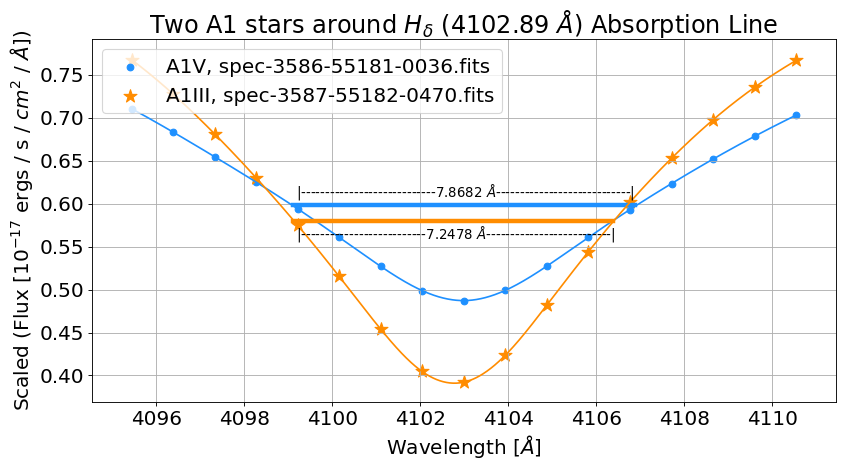
\includegraphics[width=1\linewidth]{figures/2A1.png}
	\caption{Example of the same spectral class with different wavelength width (Full Width Half Max) for the same absorption line for different MK classes.}
	\label{fig:2A1}
\end{figure}

\begin{figure}
	\centering
	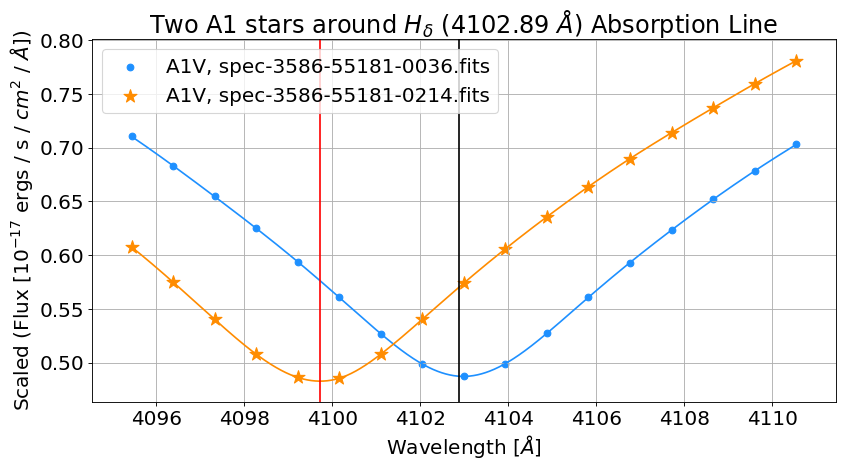
\includegraphics[width=1\linewidth]{figures/Red_Example.png}
	\caption{Example of how RV is accounted for in the feature selection window}.
	\label{fig:redP}
\end{figure}

Since there is not one absorption line that all spectral classes share, two absorption line regions are used. The two absorption lines with rest vacuum wavelengths are H$_\delta$ (4102 $\mathring{A}$) and Ca \RomanNumeralCaps{1} (4227 $\mathring{A}$). B and A stars have H$_\delta$, K and M have Ca \RomanNumeralCaps{1}, and F and G have both absorption lines. Spectral classes are separated because of the intensity of the flux in the regions and Luminosity classes are separated because of the widths of the absorption line. Figure \ref{fig:2A1} shows how the width of the absorption line changes the flux measurements for two A type stars. Using these two regions the feature matrix can be built. The flux measurements from the H$_\delta$ region and the flux measurements from the Ca \RomanNumeralCaps{1} region are combined to create a single flux array per sample, as seen in Table \ref{tab:feature-matrix2}. This feature selection must also be able to incorporate the shifting of the spectrum due to RV. Figure \ref{fig:redP} shows that with a sufficiently sized region, RV can be incorporated.

The feature matrix can be represented as an N dimensional hyper-cube.  Where each feature is a dimension in this hyper-cube. As mentioned before, the wavelengths are used as dimension labels, where the flux measurement at that wavelength is the magnitude of the vector in that dimension. This results in each reduced "spectrum" being represented as a N dimensional point. As the shape and intensity of the flux in these regions change due to spectral class, the positions of these reduced spectra change in this N dimensional hyper-cube. The same happens when the width of the absorption line changes with luminosity class.

A problem arises with the feature matrix because RV causes the flux measurements to be shifted in wavelength. This is illustrated in Table \ref{tab:example}. As mentioned earlier, each feature is unique. The problem that RV causes is that it breaks this feature uniqueness. To overcome this problem, a sufficient number of samples of the exact same class with different RV that span the range of realistic RV are required. This gives the training dataset for the classifier model sufficient samples of spectral and luminosity classes at different RV. In terms of KNN, this allows for sufficient neighbors to be nearby when classifying. In terms of RF, this forces the splitting threshold of each decision tree's node to include spectra with RV. 

% ============================================================================================================
\section{Experiments}\label{sec:exp}

In this section, the experimental setup is described and the results are presented.

% ============================================================================================================
\subsection{Experimental Setup}

The dataset used in these experiments comes from SDSS data run 14, which was collected using the BOSS spectrograph\footnote{Simplified Boss Spectrograph explanation: \url{https://www.sdss.org/instruments/boss_spectrograph/}} \citep{Smee}. Data run 14 contains a total of 335,844 spectra. Some of the data was rejected because it was not a spectral class of O, B, A, F, G, K, and M with subclass of 0 - 9 combined with luminosity class of I, II, III, IV, V, VII or that the data was missing a large portion of its spectrum, similarly to the work done in \cite{brice}. The data was also pre-processed by SDSS scientists through the methods presented by \cite{Dawson} and \cite{Stoughton}.

The usable dataset contains 168,982 stellar spectra and 46 of the 420 class combinations. It is important to note that this is real collected data and not simulated data. The spectra are first pre-processed by scaling the flux to ensure that similar classes have similar flux measurements using eq. (\ref{eq:scale}).

Then feature selection is performed using Algorithm \hyperlink{alg:FS}{1}, where bounds is the number of flux measurements before and after the absorption line. Bounds is set to 8 to cover the RV range of -552 km/s to 552 km/s and ensure that sufficient flux measurements are recorded. This results in a region of 17 flux measurements around the $H_\delta$ (4102 $\mathring{A}$) and a region of 17 flux measurements around the Ca \RomanNumeralCaps{1} (4227 $\mathring{A}$) absorption line, which is combined to form a 34 dimension feature matrix.

% I could not get the algorithm section / code to generate in aasTex. I took a picture of it and found a hyper link work around so it looks like it works.
% ----------------------------------------------------
\begin{figure*}
	\hypertarget{alg:FS}
	\centering
	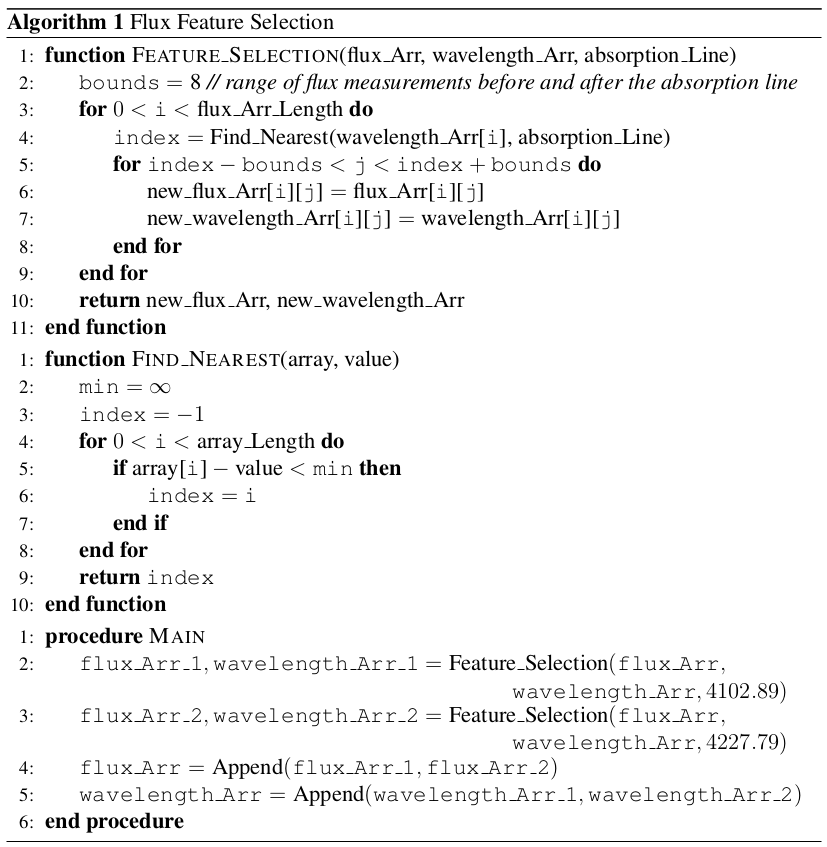
\includegraphics[width=.75\linewidth]{figures/Algorithm1.png}
	\label{alg:FS}
\end{figure*}

After the feature selection phase, the dataset is split into 2 subsets for RV. One for RV less than 200 km/s and one for RV greater than 200 km/s. Each subset is again divided into 10 subsets for 10 fold cross validation \citep{KCV}. One subset from each RV set is taken as testing sets respectively. The remaining subsets are combined into one training set. Due to the dataset being imbalanced (Figure \ref{fig:dist_B}), the training set is balanced using a \textit{Undersampling} method \citep{Japkowicz} (randomly removing samples), an \textit{Oversampling} method (randomly duplicating samples using SMOTE \citep{SMOTE}), and a \textit{Hybrid} method (Undersampling + Oversampling). Then, KNN and RF classifiers are applied to the training set and tested using the RV less than 200 km/s test set and RV greater than 200 km/s test set as well as a combined test set. These steps are repeated 10 times with different subsets used for testing for 10 fold cross validation. The accuracy, precision, recall, and F1 score (defined below) are averaged over each cross validation. Misclassification costs for incorrectly classifying a spectrum is not explored.

\newpage % Page Placement || Can be removed
\vspace*{1.5cm} % Page Placement || Can be removed
The experiments are implemented in Python, using scikit-learn \citep{scikit-learn}. Due to the size of the  dataset (16.7 GB, which is larger than the RAM used in these experiments), the Python NumPy memmap\footnote{Memmap: \url{https://docs.scipy.org/doc/numpy-1.14.0/reference/generated/numpy.memmap.html}} \citep{numpy} module was used to read very large arrays from storage rather than RAM. The experiments are performed on a personal computer with the following relevant specifications: AMD Ryzen 7 1800x 16 logical core CPU, 16 GB RAM, and 1 TB Samsung 860 EVO Solid State Drive. 


       % Distribution of classes in dataset
        \begin{figure}
	  
*{1.5cm} % Page Placement || Can be removed
            \centering
            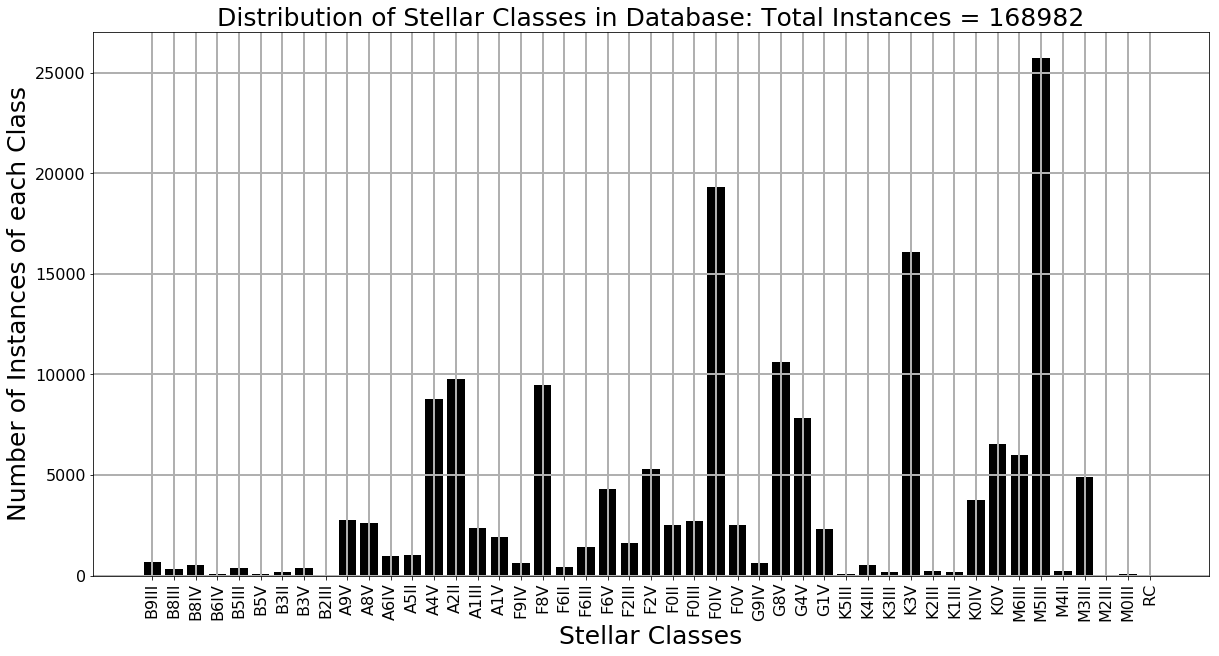
\includegraphics[width=1\linewidth]{figures/Distribution_B.png}
            \caption{Distribution of classes in the dataset. RC = Remaining Classes of 0 instances}
            \label{fig:dist_B}
        \end{figure}

\newpage % Page Placement || Can be removed
KNN and RF use the scikit-learn default parameters \citep{scikit-learn}. Precision\footnote{Precision SciKit-Learn: \url{https://scikit-learn.org/stable/auto_examples/model_selection/plot_precision_recall.html}}, recall\footnote{Recall SciKit-Learn: \url{https://scikit-learn.org/stable/modules/generated/sklearn.metrics.recall_score.html\#sklearn.metrics.recall_score}}, and F1 score\footnote{F1 Score SciKit-Learn: \url{https://scikit-learn.org/stable/modules/generated/sklearn.metrics.f1_score.html\#sklearn.metrics.f1_score}} are computed using functions implemented by the scikit-learn sklearn.metrics package \citep{scikit-learn}. Feature selection is implemented using Algorithm \hyperlink{alg:FS}{1} in Python and uses the Python multiprocessing package\footnote{Multiprocessing: \url{https://docs.python.org/3.7/library/multiprocessing.html\#module-multiprocessing}} for parallelization. 

Precision is the measure of how well a predicted class compares to actual classes. \citep{Marsland}. For example, in the binary class case, precision is the number of samples correctly predicted as class 1 divided by the total number of samples predicted as class 1 (eq. \ref{eq:p}). Recall is the measure of how well an actual class compares to predicted classes. \citep{Marsland}. For example, in the binary class case, recall is the number of samples correctly predicted as class 1 divided by the total number of samples that are actually class 1 (eq. \ref{eq:r}). F1 score is a type of harmonic mean that combines precision and recall into a single metric (eq. \ref{eq:f}) \citep{Marsland}. The closer precision, recall, and F1 score is to 1, the more accurate the model. In terms of this work, precision, recall, and F1 score are reported as an average of all the individual precision, recall, and F1 score measurements associated with each of the 46 classes respectively. Precision, Recall, and F1 score are defined in the binary class case as follows:
\begin{equation}\label{eq:p}
	Precision = \frac{Total\_TP}{Total\_TP + Total\_FP}
\end{equation}

\begin{equation}\label{eq:r}
	Recall = \frac{Total\_TP}{Total\_TP + Total\_FN}
\end{equation}

\begin{equation}\label{eq:f}
	F_1 = 2 \frac{Precision * Recall}{Precision + Recall}
\end{equation}

\noindent where TP (True Positive) is defined as a prediction of class 1 being correctly classified as class 1, FP (False Positive) is defined as a prediction of class 1 being incorrectly classified as class 2, and FN (False Negative) is defined as a sample of class 1 being incorrectly predicted as class 2. In the multi-class problem, False Positive is defined as a prediction of class i being incorrectly classified as class $\neq$ i and False Negative is defined as a sample of class i being incorrectly predicted as class $\neq$ i. More information regarding precision, recall, and F1 score can be found here: \cite{Powers}. 


% ======= KNN =========================
% KNN results 
\begin{table*}
\centering
\caption{10-Fold cross validation Accuracy for KNN.}
\label{tab:KNND}
	\begin{tabular}{|c|c|c|c|c|c|c|c|}
		\hline
		\multirow{2}{*}{Balance Method} & \multirow{2}{*}{RV} & \multicolumn{6}{c|}{Accuracy (\%) for K Neighbors} \\       
		&  & 3.0 &   5.0 &   7.0 &   10.0 &   15.0 &   20.0 \\ \hline \hline
		 \multirow{3}{*}{Undersampled}& All & 52.66 & 52.31 & 51.47 &  50.73 &  49.63 &  48.49 \\ \cline{2-8}
		& $<$ 200 km/s	& 53.32 & 52.99 & 52.17 &  51.45 &  50.35 &  49.23 \\ \cline{2-8}
		& $\geq$ 200 km/s	& 23.97 & 22.94 & 21.18 &  19.38 &  17.98 &  16.67 \\ \hline \hline
		 \multirow{3}{*}{Hybrid}      & All & 93.02 & 92.63 & 92.31 &  91.85 &  91.26 &  90.73 \\ \cline{2-8}
		& $<$ 200 km/s	& 92.92 & 92.56 & 92.26 &  91.82 &  91.28 &  90.77 \\ \cline{2-8}
		& $\geq$ 200 km/s	& 97.15 & 95.62 & 94.44 &  92.94 &  90.54 &  88.96 \\ \hline \hline
		 \multirow{3}{*}{Oversampled} & All & 95.48 & 95.00 & 94.54 &  93.98 &  93.24 &  92.58 \\ \cline{2-8}
		& $<$ 200 km/s& 95.46 & 94.99 & 94.56 &  94.02 &  93.32 &  92.69 \\ \cline{2-8}
		& $\geq$ 200 km/s	& 96.41 & 95.28 & 93.91 &  92.18 &  89.54 &  87.78 \\ \hline
	\end{tabular}
\end{table*}

% === PRF ===============
% KNN PRF Default Oversampling
\begin{table*}
\centering
\caption{10-Fold cross validation Precision, Recall, and F1 Score for KNN using Oversampling.}
\label{tab:PRFKNND}
	\begin{tabular}{|c|c|c|c|c|c|c|c|}
		\hline
		\multirow{2}{*}{} & \multirow{2}{*}{RV} & \multicolumn{6}{c|}{K Neighbors} \\ 
		        &   &   3.0 &   5.0 &   7.0 &   10.0 &   15.0 &   20.0  \\ \hline \hline
		 \multirow{3}{*}{Precision} & All & 0.805493 & 0.795833 & 0.789050 & 0.781626 & 0.767124 & 0.756264 \\ \cline{2-8}
		& $<$ 200 km/s	 & 0.803331 & 0.793968 & 0.787575 & 0.780606 & 0.766780 & 0.756458 \\ \cline{2-8}
		& $\geq$ 200 km/s	& 0.926071 & 0.897225 & 0.872481 & 0.838610 & 0.793230 & 0.756975 \\ \hline \hline
		 \multirow{3}{*}{Recall} & All   & 0.835391 & 0.834499 & 0.834981 & 0.835475 & 0.833052 & 0.829150 \\ \cline{2-8}
		& $<$ 200 km/s	 & 0.832799 & 0.831953 & 0.832601 & 0.833312 & 0.831288 & 0.829150 \\ \cline{2-8}
		& $\geq$ 200 km/s	& 0.941410 & 0.921932 & 0.905449 & 0.879239 & 0.853662 & 0.959524 \\ \hline \hline
		 \multirow{3}{*}{F1 Score} & All & 0.811617 & 0.805477 & 0.801665 & 0.796227 & 0.786297 & 0.776893 \\ \cline{2-8}
		& $<$ 200 km/s	 & 0.809250 & 0.803309 & 0.799771 & 0.794651 & 0.785290 & 0.776297 \\ \cline{2-8}
		& $\geq$ 200 km/s	& 0.989692 & 0.985351 & 0.981322 & 0.975739 & 0.967290 & 0.827752 \\ \hline
	\end{tabular}
\end{table*}

% KNN Time Default Oversampling
\begin{table*}
\centering
\caption{10-Fold cross validation Execution Times for KNN using Oversampling for all RV.}
\label{tab:KNNT}
	\begin{tabular}{|c|c|c|c|c|c|c|}
		\hline
		\multirow{2}{*}{} & \multicolumn{6}{c|}{Time in seconds for K Neighbors} \\ 
		           &   3.0 &   5.0 &   7.0 &   10.0 &   15.0 &   20.0  \\ \hline 
		 Feature Selection & 90.89 & 90.89 & 90.89 & 90.89 & 90.89 & 90.89 \\ \hline
		 Train             &   6.91 &   6.91 &   6.95 &   6.94 &   6.88 &   6.82 \\ \hline
		 Test              &   3.03 &   3.22 &   3.41 &  3.62 &  3.92 &  4.19 \\ \hline
	\end{tabular}
\end{table*}


% ======= RF =========================
% RF results Default
\begin{table*}
\centering
\caption{10-Fold cross validation Accuracy for RF.}
\label{tab:RFD}
	\begin{tabular}{|c|c|c|c|c|c|c|c|}
		\hline
		\multirow{2}{*}{Balance Method} & \multirow{2}{*}{RV} & \multicolumn{6}{c|}{Accuracy (\%) for N Trees} \\ 
		  & &   10.0 &   50.0 &   100.0 &   150.0 &   200.0 &   250.0 \\ \hline \hline
		  \multirow{3}{*}{Undersampled} & All &  52.45 &  58.13 &   58.75 &   59.01 &   59.09 &   59.21 \\ \cline{2-8}
			& $<$ 200 km/s &  53.09 &  58.78 &   59.39 &   59.65 &   59.72 &   59.83 \\ \cline{2-8}
			& $\geq$ 200 km/s	 &  24.62 &  29.79 &   30.85 &   31.48 &   31.77 &   31.91 \\ \hline \hline
		  \multirow{3}{*}{Hybrid} & All      &  93.83 &  94.44 &   94.48 &   94.48 &   94.50 &   94.49 \\ \cline{2-8}
			& $<$ 200 km/s      &  93.73 &  94.35 &   94.38 &   94.39 &   94.41 &   94.41 \\ \cline{2-8}
			& $\geq$ 200 km/s&  98.39 &  98.36 &   98.36 &   98.44 &   98.61 &   98.41 \\ \hline \hline
		  \multirow{3}{*}{Oversampled} & All  &  96.39 &  97.05 &   97.12 &   97.16 &  97.15       &   97.16      \\ \cline{2-8}
			& $<$ 200 km/s &  96.34 &  97.01 &   97.09 &   97.13 &  97.12       &   97.12      \\ \cline{2-8}
			& $\geq$ 200 km/s	&  98.49 &  98.65 &   98.62 &   98.62 &  98.65      &   98.65      \\ \hline 
	\end{tabular}
\end{table*}

% === PRF ===============
% RF PRF results Default Oversampling
\begin{table*}
\centering
\caption{10-Fold cross validation Precision, Recall, and F1 Score for for RF using Oversampling.}
\label{tab:PRFRFD}
	\begin{tabular}{|c|c|c|c|c|c|c|c|}
		\hline
		\multirow{2}{*}{} & \multirow{2}{*}{RV}  & \multicolumn{6}{c|}{N Trees} \\ 
		  &   &  10.0 &     50.0 &    100.0 &    150.0 &    200.0 &    250.0  \\ \hline \hline
		 \multirow{3}{*}{Precision} & All & 0.827606 & 0.845460 & 0.849466 & 0.849149 & 0.850188 & 0.850051 \\ \cline{2-8}
			& $<$ 200 km/s & 0.825895 & 0.844077 & 0.848296 & 0.847941 & 0.848908 & 0.848765 \\ \cline{2-8}
			& $\geq$ 200 km/s & 0.968922 & 0.971134 & 0.967166 & 0.968655 & 0.971852 & 0.971852 \\ \hline \hline
		\multirow{3}{*}{Recall} & All    & 0.849646 & 0.862420 & 0.866250 & 0.866379 & 0.868213 & 0.868580 \\ \cline{2-8}
			& $<$ 200 km/s & 0.847837 & 0.861001 & 0.865014 & 0.865182 & 0.866917 & 0.867305 \\ \cline{2-8}
			& $\geq$ 200 km/s   & 0.973081 & 0.973082 & 0.970220 & 0.972075 & 0.972433 & 0.972433 \\ \hline \hline
		 \multirow{3}{*}{F1 Score} & All  & 0.832101 & 0.847679 & 0.851134 & 0.851346 & 0.852966 & 0.853006 \\ \cline{2-8}
			& $<$ 200 km/s & 0.830256 & 0.846204 & 0.849857 & 0.850088 & 0.851616 & 0.851663 \\ \cline{2-8}
			& $\geq$ 200 km/s  & 0.969936 & 0.970727 & 0.967720 & 0.969363 & 0.970591 & 0.970591 \\ \hline 
	\end{tabular}
\end{table*}

% RF Time Default Oversampling
\begin{table*}
\centering
\caption{10-Fold cross validation Execution Times for RF using Oversampling for all RV.}
\label{tab:RFT}
	\begin{tabular}{|c|c|c|c|c|c|c|}
		\hline
		\multirow{2}{*}{} & \multicolumn{6}{c|}{Time in seconds for N Trees} \\ 
		           &   10.0 &   50.0 &   100.0 &   150.0 &   200.0 &   250.0 \\ \hline
		 Feature Selection & 90.89 & 90.89 & 90.89 & 90.89  &    90.89     &    90.89\\ \hline
		 Train             &  129.23 & 605.32 & 1226.75 & 1857.21 &    2448.32     &    2960.94 \\ \hline
		 Test              &    0.65 &   2.91 &   6.03 &   9.16 &    11.99     &    14.46     \\ \hline
	\end{tabular}
\end{table*}

% ============================================================================================================
\section{Discussion}\label{sec:discussion}

	Tables \ref{tab:KNND} and \ref{tab:RFD} show that classification using KNN has essentially the same accuracy as RF when using hybrid and oversampling balancing. These tables demonstrate that using KNN and RF along side Algorithm \hyperlink{alg:FS}{1} for feature selection are viable options for the automated classification of stellar spectra because of the high accuracy achieved. Table \ref{tab:KNND} demonstrate that using three neighbors for KNN classification performs the best for KNN. Table \ref{tab:RFD} shows that changing the number of trees used in RF does not significantly change the classification accuracy. Tables \ref{tab:KNND} and \ref{tab:RFD} shows that Oversampling balancing outperforms Hybrid balancing. 

Tables \ref{tab:PRFKNND} and \ref{tab:PRFRFD} show that the precision and recall is less than accuracy (Tables \ref{tab:KNND} and \ref{tab:RFD}). The precision implies on average that the RF model's prediction of class i is 84.91\% (Table \ref{tab:PRFRFD}) actually class i. Where recall implies on average, the RF model predicts 86.63\% (Table \ref{tab:PRFRFD}) of the samples that is class i as class i. It is important to note that the test sets for all RV, RV $<$ 200 km/s, and RV $\geq$ 200 km/s metrics are tested using the same trained model. As seen in these tables, this approach accurately classifies both RV $<$ 200 km/s and RV $\geq$ 200 km/s. However, RV $\geq$ 200 km/s has a higher accuracy, precision, and recall (Table \ref{tab:PRFRFD}) than RV $<$ 200 km/s. This could be the result of an imbalance between low RV and high RV samples and overfitting the model in the low RV range. Future work will attempt to increase precision and recall for low RV, which includes balancing the RV range. 

Tables \ref{tab:KNNT} and \ref{tab:RFT} show the execution times for each experiment. These tables show that KNN performs much faster than RF. KNN has a faster train time than RF, but RF has a faster test time than KNN. For both KNN and RF, feature selection takes approximately the same amount of time, which is expected since they both use the same feature selection.
	
This approach takes considerably fewer steps than the one in \cite{Bolton} and produces excellent results. The execution times and the obtained accuracy demonstrate that, for a real application of this work, the automated classification of observed stellar spectra into a complete MK classification using a single classifier not only achieves a high accuracy but is also fast.

These experiments yielded an accuracy of 97.16\% for RF (Table \ref{tab:RFD}) using Oversampling Balancing and 150 decision trees (Table \ref{tab:RFD}), which is significantly better than \cite{Xing}, which reports 81.66\% accuracy for just Support Vector Machine (SVM) with no data reduction, 93.26\% for wavelet + SVM and 81.30\% for PCA + SVM.  \cite{Schierscher} are able to achieve an 85\% match in comparison with SEGUE Stellar Parameter Pipeline (SSPP) using an Artificial Neural Network (ANN), but this is not comparable since they did not classify into direct spectral and luminosity classes. \cite{Schierscher} also never addresses the fact that their data is imbalanced.

Other authors such as \cite{Bazarghan, YI, Luo} do not report metrics that are comparable to the work conducted in this paper. \cite{Bazarghan} used a Probabilistic Neural Network implemented in MATLAB and they used a $\chi^2$ value to determine classification accuracy. They make the assumption that a $\chi^2$ value of 0.002 or lower is considered classified correctly, then they achieved a success rate of about 88\% in only a few seconds. \cite{YI} find that RF performed better than the MLP with Root Mean Square Error (RMSE) of 1.04 and 1.36 respectively. \cite{Luo} separated the classification into two classifiers. For the spectral classes, the authors used a non-parameter regression method. For the luminosity classes, the authors removed or normalized the continuum of the spectra and used a partial least-squared regression method. \cite{Luo} used three spectra data sources, \cite{Silva}, \cite{Pickles}, and \cite{Jacoby}. They achieved a standard deviation for the spectral classes of $\sigma = 0.7994$ and for the luminosity classes of $\sigma = 0.58159$.

As described above in Section \ref{sec:exp}, these experiments deal with data collected by a real astronomical survey. As such, when an astronomical survey points their telescopes into the sky, they get the samples (classes) that they get. The experiments presented here deal with a subset of all possible class combinations. It is important to note that not all possible class combinations (O, B, A, F, G, K, and M with sub - classes of 0 - 9 combined with I, II, III, IV, V, VII) are common or even found in nature. Therefore, even though this approach yielded great results, there cannot be a claim that this approach will guarantee work for all stellar classes. There is, however, some theoretical validity to this approach. 

Referencing Figure \ref{fig:dist_B}, O type stars are the only spectral class not found in the dataset. Figure \ref{fig:O} shows that O type stars also contain the H$_\delta$ absorption line. Therefore, the missing spectral and luminosity classes are compatible with this approach because every spectral major class has at least one absorption line in the feature selection regions, which allows for the variation in width for luminosity classes.

%Recall that spectral classes are based on absorption lines and the luminosity classes are based on the widths of those absorption lines \citep{Gray} and according to Section \ref{sec:Approach_B}, the shape, intensity, and width of the absorption lines are \textbf{incorporated through the feature selection}. 

        \begin{figure}
            \centering
             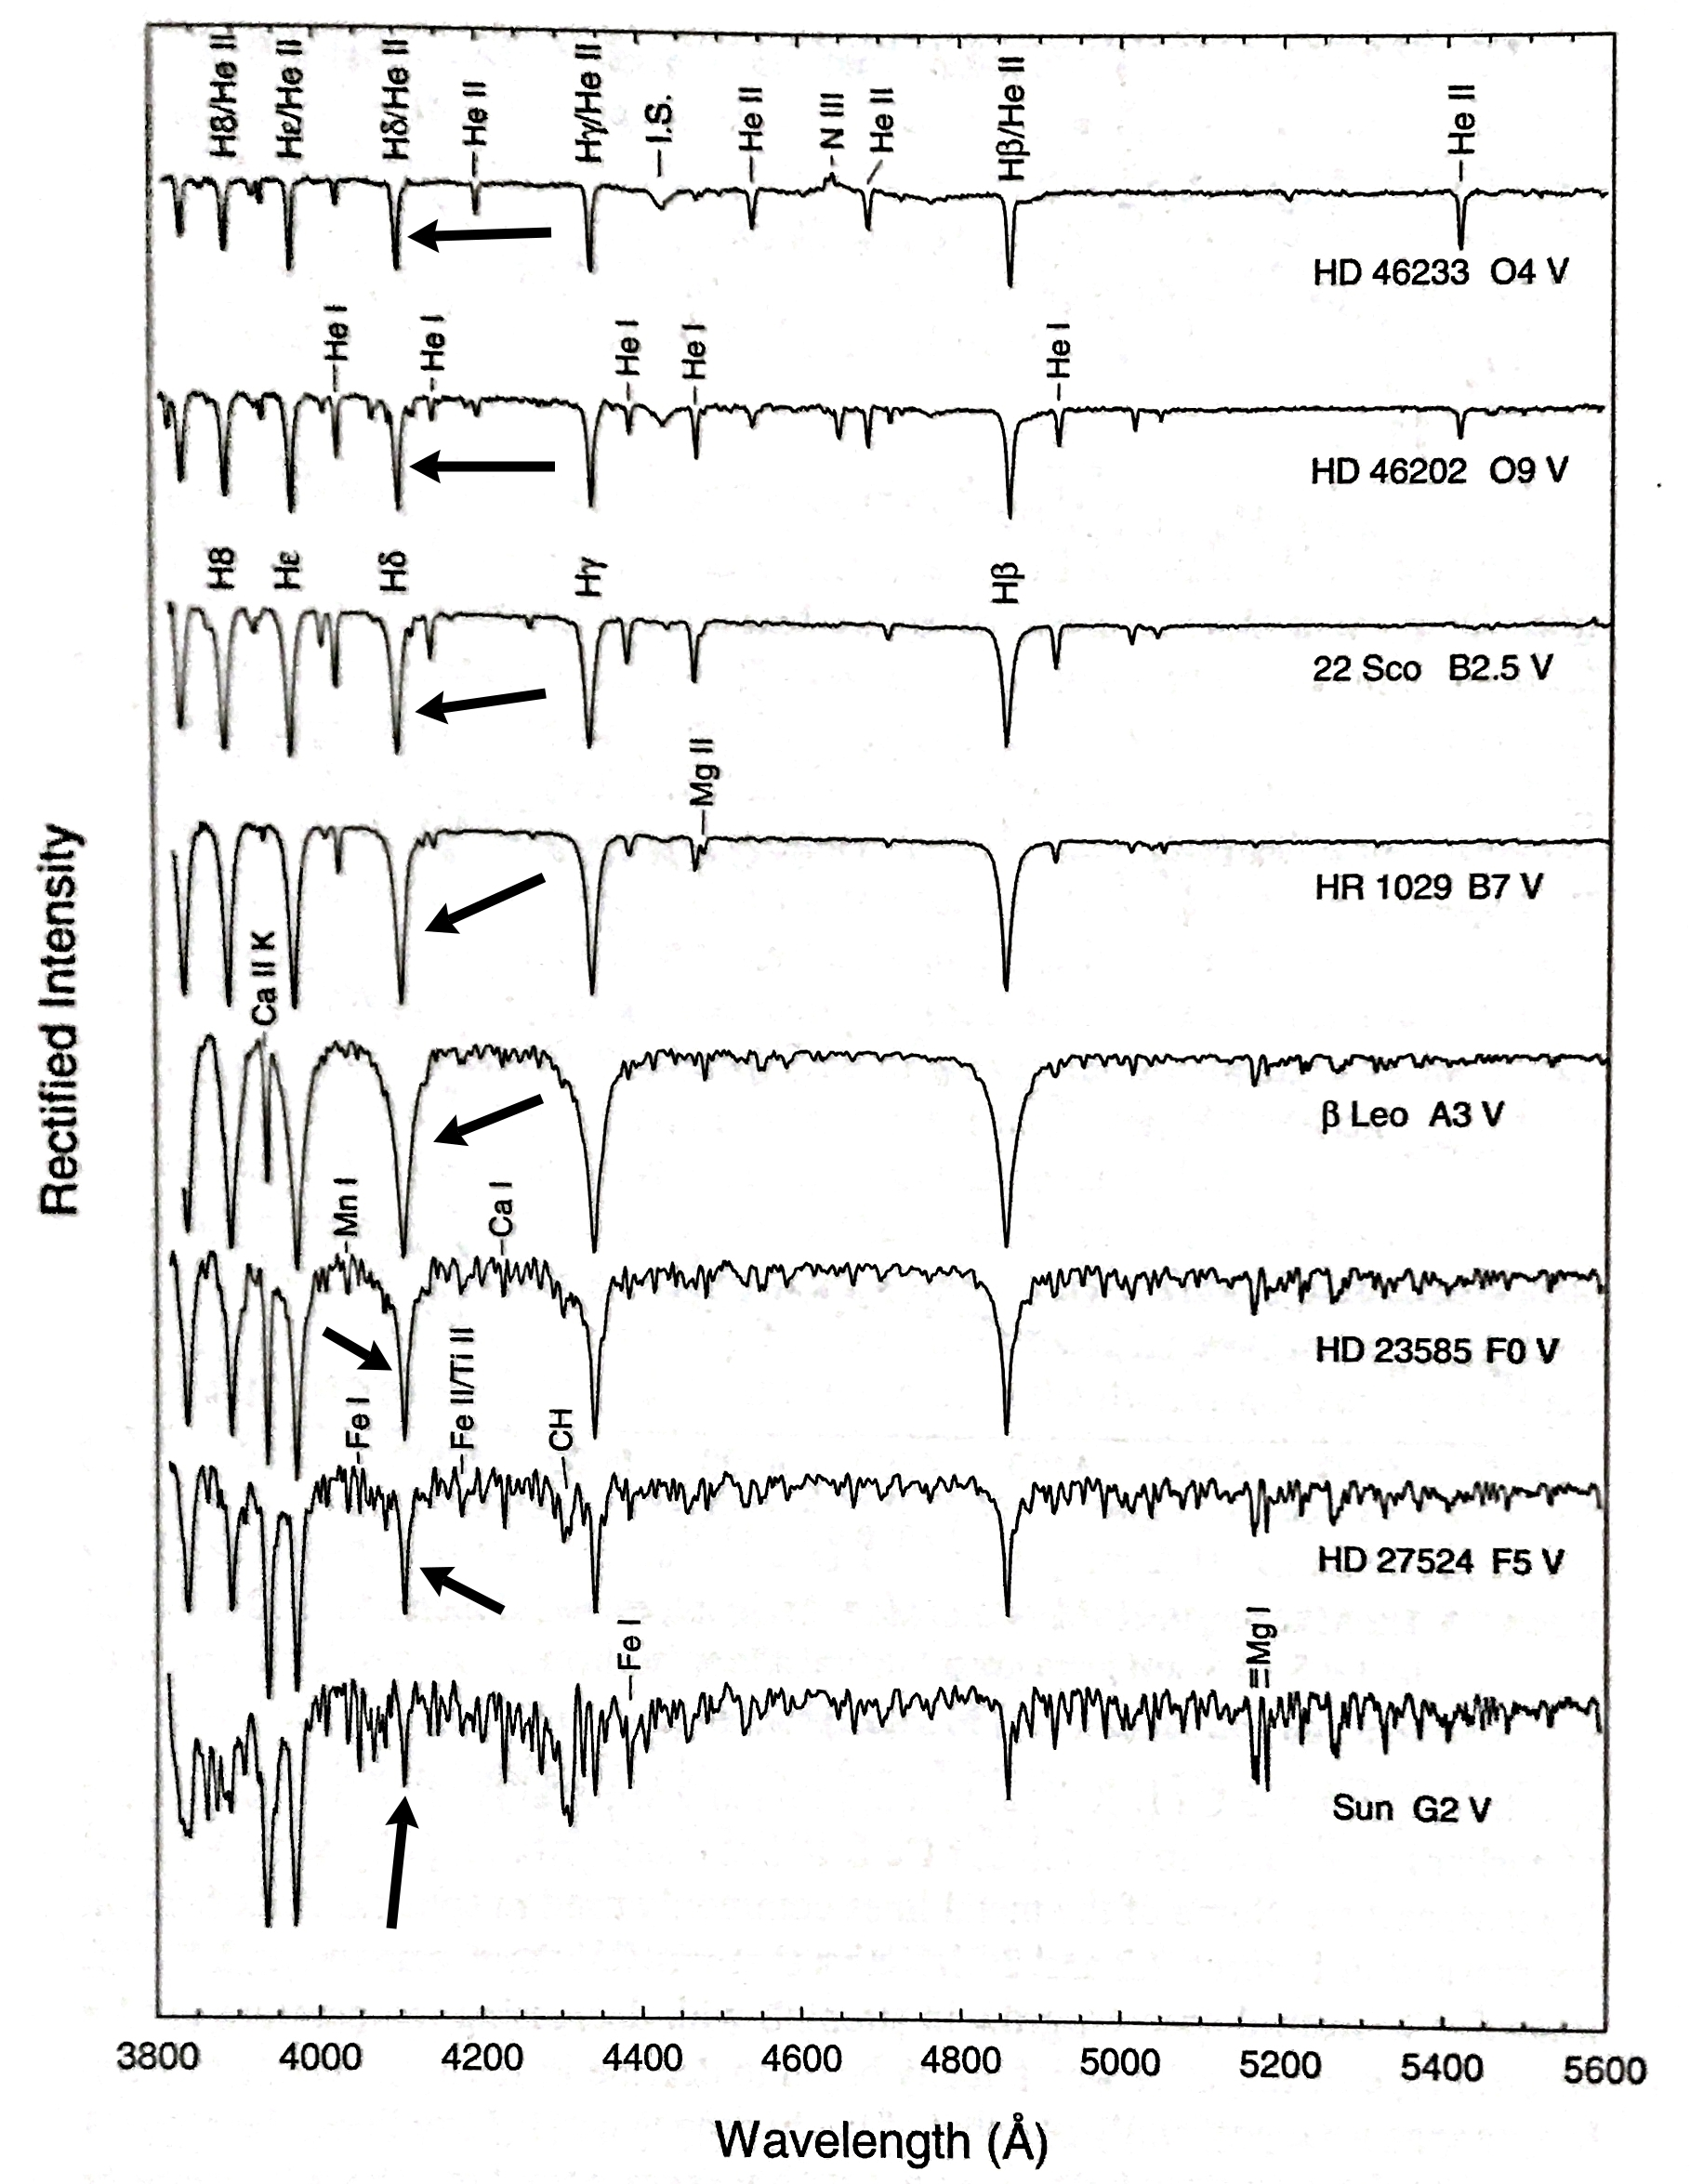
\includegraphics[width=1\linewidth]{figures/OStar.jpeg}
            \caption{Sample of continuum normalized spectra from O - G type stars, \cite{Gray}. The arrows point to the H$_\delta$ absorption line}
            \label{fig:O}
        \end{figure}



% ============================================================================================================
\section{Conclusion}\label{sec:conc}

The results shown in this paper support that accurate automatic stellar classification can be obtained using astronomical specific feature selection. Compared to previous work of other authors, there are four interesting conclusions:

\begin{enumerate}
	\item A high level of accuracy can be obtained by considering only flux measurements at wavelengths near the $H_\delta$ and Ca \RomanNumeralCaps{1} absorption lines.
	\item A complete MK classification can be identified using a single classifier with a high level of accuracy for stars with small RV (the range of $\approx \pm$ 240 km/s). However, for stars with large RV (outside the range of $\approx \pm$ 240 km/s), increasing the value of 			bounds in Algorithm \hyperlink{alg:FS}{1} should compensate for large RV, but at the cost of an increase to the computational time because of the increase in dimensions. 
	\item Correcting for RV is not necessary because of a sufficient distribution of samples with different RV.
	\item Aside from flux scaling, any additional spectrum pre-processing after recombining and re-binning the spectra as presented by \cite{Dawson} and \cite{Stoughton} is unnecessary for SDSS stellar spectra. 

\end{enumerate}

Therefore, this new approach for the automatic classification of stellar spectra is feasible, useful, and accurate. Future work will be conducted with the concepts of this approach to automatically classify stars and large redshift objects such as galaxies and quasars. Future work will also include building the training set with an equal distribution of RV and experiment using SMOTE or similar algorithms to build a training set using a small number of real samples to simulate how this approach could work for a new spectroscopic survey.


% ============================================================================================================
\bibliography{references}

\end{document}